% Discuss preliminaries for time series modeling? 
% \section{Method: State-Space Time-Series Modeling with \ourmethod{}}

\section{Method: \ourmethod{}}
\label{sec:method_spacetime}
%

We now present \ourmethod{}, a deep architecture that uses structured state-spaces for more effective time-series modeling.
%
\ourmethod{} is a standard multi-layer encoder-decoder sequence model, built as a stack of repeated layers that each parametrize multiple SSMs. We designate the last layer as the ``decoder'', and prior layers as ``encoder'' layers. 
Each encoder layer processes an input time series sample as a sequence-to-sequence map. The decoder layer then takes the encoded sequence representation as input and outputs a prediction (for classification) or sequence (for forecasting). 

Below we expand on our contributions that allow \ourmethod{} to improve expressivity, long-horizon forecasting, and efficiency of time series modeling.
%
In Sec.~\ref{sec:expressive_ssm_layer}, we present our key building block, a layer that parametrizes the \emph{companion matrix} SSM (companion SSM) for expressive autoregressive modeling. 
% We first discuss how the companion SSM provides a highly expressive model for time series, proving that it can represent multiple fundamental processes. We then go over how we represent and compute multiple SSMs in each \ourmethodunit{}. We finally show how the companion SSM's expressiveness allows a \ourmethodunit{} to perform various standard time series data preprocessing operations simply as a forward pass via specific weight initializations.
%
In Sec.~\ref{sec:forecasting_ssm}, we introduce a specific instantiation of the companion SSM to flexibly forecast long horizons. 
% We show how (i) computing an SSM's outputs as a recurrence and (ii) explicitly training an SSM to predict future time-steps of its \emph{layer-specific} input sequences enables \ourmethod{}'s decoder to dynamically forecast arbitrary horizon lengths in a multi-layer network.
% time complexity
%
In Sec.~\ref{sec:efficient_algorithm}, we provide an efficient inference algorithm that allows \ourmethod{} to train and predict over long sequences in sub-quadratic time and space complexity. 
%
% Together these contributions make \ourmethod{} a highly modular architecture, where simply via specific weight initializations, we can efficiently compute multiple autoregressive outputs and perform built-in data preprocessing in a single forward pass.

\begin{figure}[!t]
  \centering
%   \includegraphics[width=1\textwidth]{_ICLR2023_paper/figures/figure_system_v1.pdf}
    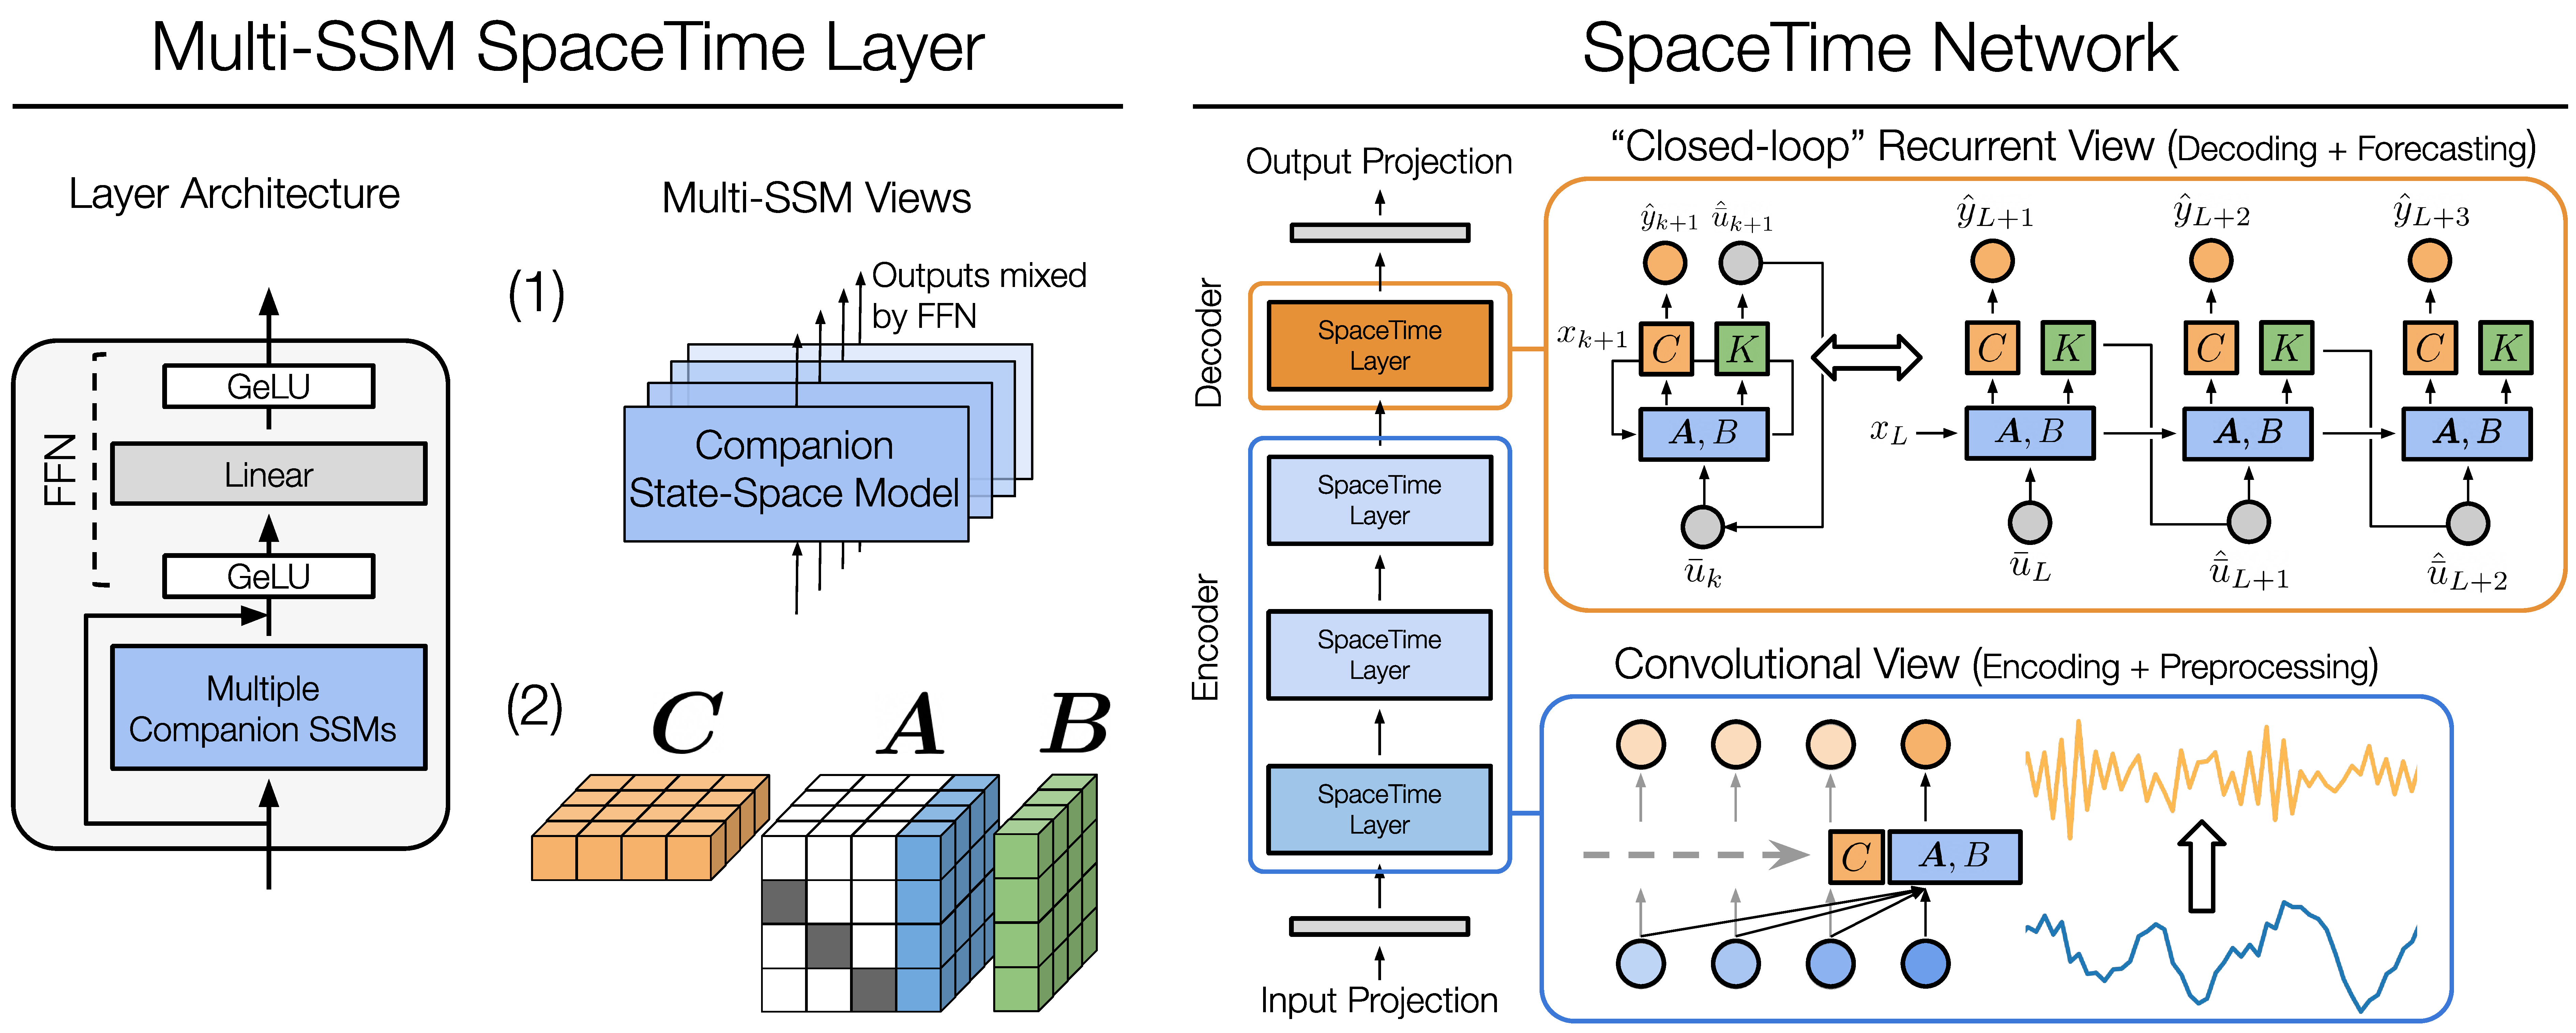
\includegraphics[width=1\textwidth]{_ICLR2023_paper/figures/space_time_architecture_v2_flipped.pdf}
%   \caption{\small \textbf{\ourmethod{} architecture overview}. The left figure displays the \ourmethod{} architecture, which is a stack on SSM layers. The middle figure expands on an SSM layer, which consists of $h$ SSMs, each of which convolves the previous layer's output sequence with the SSM kernel $\cK_L(\zA,B,C)$. On the right, we expand on the SSM kernel which is a krylov function, where the state matrix $A$ is the expressive companion matrix. \KS{update caption}}
  \caption{ \textbf{\ourmethod{} architecture and components}. \textbf{(Left):} Each \ourmethodunit{} carries weights that model multiple companion SSMs, followed optionally by a nonlinear FFN. The SSMs are learned in parallel (1) and computed as a single matrix multiplication (2). 
  %
  \textbf{(Right):} We stack these layers into a \ourmethod{} network, where
  earlier layers compute SSMs as convolutions for fast sequence-to-sequence modeling and data preprocessing, while a decoder layer computes SSMs as recurrences for dynamic forecasting.}
  \label{fig:arch_overview} 
\end{figure}


\subsection{The Multi-SSM \ourmethodunit{}}

\label{sec:expressive_ssm_layer}
% In this section, we discuss the \ourmethodunit{} layer, a linear layer with weights that parameterize multiple SSMs. We describe the key 
% We first discuss how the companion SSM provides a highly expressive model for time series, proving that it can represent multiple fundamental processes. We then discuss how we represent and compute multiple SSMs in each \ourmethodunit{}. We finally describe how specific weight initializations of the same layer architecture allow us to build-in standard data preprocessing operations useful for time series modeling. 
We discuss our first core contribution and key building block of our model, the \ourmethodunit{}, which captures the \emph{companion SSM}'s expressive properties, and prove that the SSM represents multiple fundamental processes. 
% is a linear layer with weights that parametrize the matrices of a companion SSM. 
%We first motivate the companion SSM by discussing the SSM's unique expressiveness for time series data, and prove that the SSM represents multiple fundamental processes. 
To scale up this expressiveness in a neural architecture, we then go over how we represent and compute multiple SSMs in each \ourmethodunit{}. We finally 
% describe specific instantiations of the companion SSM that we use in encoder \ourmethodunit{}s; in particular we 
show how the companion SSM's expressiveness allows us to build in various time series data preprocessing operations in a \ourmethodunit{} via different weight initializations of the same layer architecture. 
%Together these contributions make \ourmethod{} a highly modular architecture where we can efficiently compute multiple autoregressive outputs and perform built-in data preprocessing in a single forward pass.


\subsubsection{Expressive State-Space Models with the Companion Matrix}
\label{sec:expressive_ssm_with_companion}
For expressive time series modeling, our SSM parametrization represents the state matrix $\zA$ as a companion matrix.
%
Our key motivation is that $\zA$ should allow us to capture autoregressive relationships between a sample $u_k$ and various past samples $u_{k - 1}, u_{k - 2}, \ldots, u_{k - n}$.
Such dependencies are a basic yet essential premise for time series modeling; they underlie many fundamental time series processes, \eg{} those captured by standard ARIMA models.
For example, consider the simplest version of this, where $u_k$ is a linear combination of $p$ prior samples
(with coefficients $\phi_1, \ldots, \phi_p$)
% with coefficients $\{\phi_i\}_{i=1}^p$
\begin{equation}
    u_k = \phi_1 u_{k - 1} + \phi_2 u_{k - 2} + \ldots \phi_p u_{k - p}
\label{eq:ar_p_model}
\end{equation}
\ie{} a noiseless, unbiased $\text{AR}(p)$ process in standard ARIMA time series analysis~\citep{box1970time}.

To allow (\ref{eq:input_output_ts_equal}) to express (\ref{eq:ar_p_model}), we need the hidden state $x_{k}$ to carry information about past samples.
%Recall from (\ref{eq:discrete_ssm_state}) that this is controlled by $\zA$ and $\zB$. 
However, while setting the state-space matrices as trainable neural net weights may suggest we can learn arbitrary task-desirable $\zA$ and $\zB$ via supervised learning, prior work showed this could not be done without restricting $\zA$ to specific classes of matrices~\citep{gu2021combining, gupta2022diagonal}.  
% Furthermore, we prove in Proposition~\ref{} that prior proposed state-matrix classes still cannot capture this desired autoregressive behavior. 

Fortunately, we find that a class of relatively simple $\zA$ matrices suffices. We propose to set $\zA \in \mathbb{R}^{d \times d}$ as the $d \times d$ \emph{companion matrix}, a square matrix of the form:
\begin{equation}
    (\textbf{Companion Matrix})
    \;\;\;
    \zA = 
    \begin{bmatrix}
    0  & 0  & \ldots & 0 & a_{0} \\
    1 & 0  &\ldots & 0 & a_{1} \\ 
    0 & 1 & \ldots & 0 & a_{2} \\
    \vdots &    & \ddots  & \vdots  & \vdots \\
    0 & 0  & \ldots & 1 & a_{d - 1} \\
    \end{bmatrix}
    \;\;\;
    \text{\ie{}}
    \;\;\;
    \zA_{i, j} = 
    \begin{cases}
    1 & \text{for } i - 1 = j\\
    a_i & \text{for } j = d - 1\\
    0 & \text{otherwise}
    \end{cases}
    % \;\;\;\;\;(\textbf{Companion Matrix})
\label{eq:companion_matrix}
\end{equation}
Then simply letting state dimension $d = p$, assuming initial hidden state $x_0 = 0$, and setting 
\[
a := 
\begin{bmatrix}
a_0 & a_1 & \ldots & a_{d-1}
\end{bmatrix}^T
= \boldsymbol{0}, 
\;\; 
\zB = 
\begin{bmatrix}
1 & 0 & \ldots & 0
\end{bmatrix}^T, 
\;\; 
\zC = 
\begin{bmatrix}
\phi_1 & \ldots & \phi_p
\end{bmatrix}
\]
allows the discrete SSM in (\ref{eq:discrete_ssm_state}, \ref{eq:discrete_ssm_output}) to recover the $\text{AR}(p)$ process in (\ref{eq:ar_p_model}). 
%
We next extend this result in Proposition~\ref{prop:ssm_companion_expressiveness_td_bluf}, proving in App.~\ref{appendix:theory} that setting $\zA$ as the companion matrix allows the SSM to recover a wide range of fundamental time series and dynamical system processes beyond the $\text{AR}(p)$ process.
%

\begin{prop}
    % An SSM with a companion state matrix can represent ARIMA \citep{box1970time}, exponential smoothing \citep{winters1960forecasting,holt2004forecasting}, controllable linear time--invariant systems \citep{chen1984linear}.
    A companion state matrix SSM can represent ARIMA \citep{box1970time}, exponential smoothing \citep{winters1960forecasting,holt2004forecasting}, and controllable linear time--invariant systems \citep{chen1984linear}.
\label{prop:ssm_companion_expressiveness_td_bluf}
\end{prop}

% \begin{proof}
% See Appendix~\ref{appendix:theory}. 
% \end{proof}
%
As a result, by training neural network layers that parameterize the companion SSM, we provably enable these layers to learn the ground-truth parameters for multiple time series processes. In addition, as we only update $a\in \mathbb{R}^{d}$ (\ref{eq:companion_matrix}), we can efficiently scale the hidden-state size to capture more expressive processes with only $O(d)$ parameters. 
Finally, by learning multiple such SSMs in a single layer, and stacking multiple such layers, we can further scale up expressivity in a deep architecture. 

\header{Prior SSMs are insufficient} We further support the companion SSM by proving that existing related SSM representations used in 
% S4 \cite{gu2021efficiently} and S4D~\cite{gupta2022diagonal, gu2022parameterization}, 
% smith2022simplified, alcaraz2022diffusion},
\cite{gu2021efficiently, gupta2022diagonal, smith2022simplified, alcaraz2022diffusion}
% (\ie{} the \textbf{Linear State-Space Layer} proposed by \cite{gu2021combining}), 
% \citep{gu2021combining, gupta2022diagonal, smith2022simplified, alcaraz2022diffusion} 
% we further support our introduction of the companion SSM by proving that all existing such models use representations that 
\emph{cannot} capture the simple yet fundamental $\text{AR}(p)$ process. Such works, including S4 and S4D, build on the \emph{Linear State-Space Layer} (LSSL)~\citep{gu2021combining}, and cannot represent AR processes due to their continuous-time or diagonal parametrizations of $\zA$.
\begin{prop}
    No class of continuous-time LSSL SSMs can represent the noiseless $\text{AR}(p)$ process.  
\label{prop:continuous_ssm_no_ar_td_bluf}
\end{prop}
We defer the proof to App.~\ref{appendix:companion_expressivity}.
% We derive that such works, building on the  
In Sec.~\ref{sec:empirical_expressivity}, we empirically support this analysis, showing that these prior SSMs fit synthetic AR processes less accurately than the companion SSM. This suggests the companion matrix resolves a fundamental limitation in related work for time series.
% modeling.
% the companion SSM is \emph{as expressive}
%

% \begin{proof}
% \MZ{Note solution to continuous SSM is $x(k) = e^Ak x(0) + \sum_{0}^{k}e^{A(k - t)} Bu(t) dt$, and AR(p) process discrete SSM has $A$ as the shift matrix $S$. But $S \neq e^A$ for any matrix $A$}
% \end{proof}

\subsubsection{Layer Architecture and Multi-SSM Computation}
\label{sec:method_spacetime_layer}

\header{Architecture} 
To capture and scale up the companion SSM's expressive and autoregressive modeling capabilities, we model multiple companion SSMs in each \ourmethodunit{}'s weights.
% We represent the matrices of multiple companion SSMs as weights in a linear neural net layer.
\ourmethodunit{}s are similar to prior work such as LSSLs, with $\zA$, $\zB$, $\zC$ as trainable weights, and $\zD$ added back as a skip connection. To model multiple SSMs, we add a dimension to each matrix. For $s$ SSMs per \ourmethodunit{}, we specify weights $\zA \in \mathbb{R}^{s \times d \times d}$, $\zB \in \mathbb{R}^{d \times s}$, and $\zC \in \mathbb{R}^{s \times d}$. Each slice in the $s$ dimension represents an individual SSM. We thus compute $s$ outputs and hidden states in parallel by following (\ref{eq:discrete_ssm_state}) and (\ref{eq:discrete_ssm_output}) via simple matrix multiplications on standard GPUs.

% \header{\ourmethod{} block} 
To model dependencies across individual SSM outputs, 
% or different features in a multivariate time series sample input, 
we optionally follow each \ourmethodunit{} with a one-layer nonlinear feedforward network (FFN). The FFN thus mixes the $m$ outputs across a \ourmethodunit{}'s SSMs, allowing subsequent layers to model dependencies across SSMs. 

% --------------------
% Move to appendix or explain briefly in results
% --------------------
% For time series classification, the last layer FFN projects the $m$ outputs across the SSMs to the number of classes $c$, resulting in $\boldsymbol{y'} \in \mathbb{R}^{L \times c}$. We then perform standard pooling strategies across the time dimension (e.g., averaging) to retrieve the final output class logits $\boldsymbol{y} \in \mathbb{R}^c$. For time series forecasting, we obtain the final outputs using a closed-loop SSM discussed in Sec. \ref{sec:forecasting_ssm}.


\header{Computation} 
To compute the companion SSM, we could use the recurrence in (\ref{eq:discrete_ssm_state}). However, this sequential operation is slow on modern GPUs, which parallelize matrix multiplications.
%
Luckily, as described in \cite{gu2021efficiently} we can also compute the SSM as a \textbf{1-D convolution}. This enables parallelizable inference and training. 
To see how, note that given a sequence with at least $k$ inputs and hidden state $x_0 = 0$, the hidden state and output at time-step $k$ by induction are:

\begin{equation}
x_{k} = \sum_{j = 0}^{k - 1}\zA^{k - 1 - j} \zB u_j \;\;\;\text{and}\;\;\;
    y_k = \sum_{j = 0}^{k - 1} \zC \zA^{k - 1 - j} \zB u_j 
\label{eq:convolution_view}
\end{equation}

We can thus compute hidden state $x_k$ and output $y_k$ as 1-D convolutions with ``filters'' as
\begin{align}
    \zF^x &= (\zB, \zA \zB, \zA^2 \zB, \ldots, \zA^{\ell - 1} \zB) & (\text{Hidden State Filter}) \label{eq:state_filter}\\
    \zF^y &= (\zC\zB, \zC\zA \zB, \zC\zA^2 \zB, \ldots, \zC\zA^{\ell - 1} \zB) & (\text{Output Filter}) \label{eq:output_filter} \\
% \end{align}
% \vspace{-0.5cm}
% \begin{align}
\centering
    x_k &= (\zF^x * \zu)[k] \;\;\;\text{and}\;\;\; y_k = (\zF^y * \zu)[k] \label{eq:convolution_output}
\end{align}
So when we have inputs available for each output (\ie{} equal-sized input and output sequences) 
% when processing an input time series sequence with an encoder \ourmethodunit{}, 
we can obtain outputs by first computing output filters $\zF^y$ (\ref{eq:output_filter}), and then computing outputs efficiently with the Fast Fourier Transform (FFT). We thus compute each encoder SSM as a convolution.

For now we note two caveats. Having inputs for each output is not always true, \eg{} with long horizon forecasting. Efficient inference also importantly requires that $\zF^y$ can be computed efficiently, but this is not necessarily trivial for time series: we may have long input sequences with large $k$. 

Fortunately we later provide solutions for both. In Sec.~\ref{sec:forecasting_ssm}, we show how to predict output samples many time-steps ahead of our last input sample via a ``closed-loop'' forecasting SSM. In Sec.~\ref{sec:efficient_algorithm} we show how to compute both hidden state and output filters efficiently over long sequences via an efficient inference algorithm that handles the repeated powering of $\zA^k$.  


\subsubsection{Built-in Data Preprocessing with Companion SSMs}
\label{sec:preprocessing_ssms}

% \header{Preprocessing SSMs} 
We now show how beyond autoregressive modeling, the companion SSM also enables \ourmethodunit{}s to do
% We now discuss how the companion SSM enables 
standard data preprocessing techniques used to handle nonstationarities. 
% By dedicating certain SSMs in earlier encoder layers as ``preprocessing'' SSMs, we can easily incorporate popular preprocessing operations to extract useful time series features in a \ourmethod{} model.
% without overly-specialized architectures. 
%
% 
Consider differencing and smoothing, two classical techniques to handle nonstationarity and noise:
% \begin{align}
% u_k' &= u_{k} - u_{k - 1} & \text{(1st-order differencing)} \\ 
% u_k' &= \frac{1}{m} \sum_{i = 0}^{m - 1} u_{k - i} & \text{($m$-order moving average smoothing)}
% \end{align}
% \[
% u_k' = u_{k} - u_{k - 1}\; \text{(1st-order differencing)} \;\Big{\lvert{}}\;
% u_k'&= \textstyle \sum_{i = 0}^{\textcolor{blue}{n} - 1} u_{k - i} / \textcolor{blue}{n}\; \text{($\textcolor{blue}{n}$-order moving average smoothing)}
% \]
\[
u_k' = u_{k} - u_{k - 1}\; \text{(1st-order differencing)} \;\Big{\lvert{}}\;
u_k' = \frac{1}{n} \sum_{i = 0}^{n - 1} u_{k - i} \; \text{($n$-order moving average smoothing)}
\]
%
% Many classical methods require these operations to work well, \eg{} differencing in ARIMA~\citep{box1970time}). Recent deep learning methods also try to incorporate similar inductive biases, but via specialized and dedicated architectures~\citep{woo2022etsformer}. 
% %
% While we could in principle learn to extract similar features by treating the SSM as black-box, end-to-end training may not recover these useful features in practice.  
%
%
We explicitly build these preprocessing operations into a \ourmethodunit{} by simply initializing companion SSM weights. Furthermore, by specifying weights for multiple SSMs, we simultaneously perform preprocessing with various orders in one forward pass. 
%
We do so by setting $\boldsymbol{a} = \boldsymbol{0}$ and $\zB = [1, 0, \ldots, 0]^T$, such that SSM outputs via the convolution view (\ref{eq:convolution_view}) are simple sliding windows / $1$-D convolutions with filter determined by $\zC$. We can then recover
arbitrary $n$-order differencing or average smoothing via $\zC$ weight initializations, \eg{} (see App.~\ref{appendix:specific_ssm_parameterizations} for more examples),
\begin{align}
%   C &= \begin{bmatrix} 1 & -1 & 0 & \;\;\;0 & 0 & \ldots & 0 \end{bmatrix} & (\text{First-order Differencing})\\
%   C &= \begin{bmatrix} 1 & -2 & 1 & \;\;\;0 & 0 & \ldots & 0\end{bmatrix} & (\text{Second-order Differencing})\\
%   C &= \begin{bmatrix} 1 & -3 & 3 & -1 & 0 & \ldots & 0\end{bmatrix} & (\text{Third-order Differencing})\\
%     C &= \begin{bmatrix} \frac{1}{m} & \ldots & \frac{1}{m} & 0&  0 & \ldots & 0\end{bmatrix} & (\text{Moving average of size $m$})\\
    \zC = 
    \begin{bmatrix}
    % 1 & -1 & 0 & \phantom{-}0 & 0 & \ldots & 0 \\
    1 & -2 & 1 & \phantom{-}0 & 0 & \ldots & 0 \\
    %1 & -3 & 3 & -1 & 0 & \ldots & 0 \\
    1/n & \ldots & 1/n & \phantom{-}0 & 0 & \ldots & 0 \\
    \end{bmatrix}
    \;\;\;\;\;\;
    \begin{matrix}
    % \hfill\text{(1st-order differencing)} \\
    \hfill\text{ (2nd-order differencing)} \\
    %\hfill\text{ (3rd-order differencing)} \\
    \hfill\text{ ($n$-order moving average smoothing)}
    \end{matrix}
\end{align}
% The companion SSM thus enables various preprocessing techniques with the same general layer architecture. 
%We show how to recover additional operations, such as \emph{exponential smoothing}, in App.~\ref{appendix:theory}. 
% We leave recovering other operations for future work. 
% For simplicity we only use differencing and simple moving average smoothing SSMs. 



% we can also recover 

% By training the  inheriting the expressive autoregressive modeling properties of the companion SSM

% this multi-SSM layer then inherits the expressive autoregressive modeling properties of the companion SSM, and we 

% We now further show we can recover through two specific instantiations of the SSM. 

% We use this default multi-SSM layer in each ``encoder'' layer of a \ourmethod{} network.

% By default, we can

% across individual SSM outputs, or different features in multivariate time series. 

% --- MOVED TO APPENDIX --- 
% Furthermore, in Appendix~\ref{appendix:todo} we show that with the companion matrix we \emph{do not lose} any modeling expressiveness compared to prior SSMs.

% %
% Finally, we show in Prop.~\ref{prop:companion_as_expressive_as_diagonal} that learning discrete SSMs with a companion state-matrix (henceforth ``companion SSMs'') is a modeling choice \emph{as expressive} as that of many prior proposed SSMs, which restrict $\zA$ to be diagonal. This is because a subset of all companion matrices are also diagonalizable.
% % (if $\boldsymbol{a} \neq \boldsymbol{0}$).
% %
% \begin{prop}
%     The companion SSM is as expressive as any diagonal-$\zA$ SSM.
% \label{prop:companion_as_expressive_as_diagonal}
% \end{prop}
% \begin{proof}
% \MZ{}
% \end{proof}
% %

% Together, Prop.~\ref{prop:ssm_companion_expressiveness},~\ref{prop:continuous_ssm_no_ar},~\ref{prop:companion_as_expressive_as_diagonal} suggest that our proposed companion SSM is uniquely expressive for time series modeling, while inheriting the expressive benefits of prior LSSL formulations (learning $A, B, C$ as neural net weights).
% %
% We thus learn SSMs with the companion state-matrix, training a neural net that parameterizes and updates $\boldsymbol{a}\in \mathbb{R}^{d \times 1}$ in (\ref{eq:companion_matrix}).
% %
% To train and forecast efficiently over long time series sequences, we next show how we can compute hidden states and outputs efficiently.
% We next show how we can compute hidden states and outputs efficiently with this representation for fast inference and training.

% \KS{should we add note on long-range dependencies here?}





%

%

%

%

%
\subsection{Long Horizon Forecasting with Closed-loop SSMs}
\label{sec:forecasting_ssm}

We now discuss our second core contribution, which enables long horizon forcasting. Using a slight variation of the companion SSM, we allow the same constant size \ourmethod{} model to forecast over many horizons. This \emph{forecasting SSM} recovers the flexible and stateful inference of RNNs, while retaining the faster parallelizable training of computing SSMs as convolutions. 

% We first describe challenges and limitations with forecasting for deep nets. We then show how introducing a \emph{closed-loop} view of SSMs enables \ourmethod{}'s decoder to dynamically forecast specified horizons in a multi-layer network. The key idea is to 
% % (i) computing SSM outputs as a recurrence and (ii) 
% explicitly train \ourmethod{}'s last-layer SSMs to predict future time-steps of both the observed time series sequence (as a standard open-loop system) and its \emph{layer-specific} inputs (as a closed-loop counterpart). 

% Note: for related work, add a line that talks about how most sota time series neural networks use "direct multi-step forecasting", which is in contrast to what we do.We therefore get stateful, constant model size. But others scale to many more parameters.
\header{Challenges and limitations} For forecasting, a model must process an input lag sequence of length $\ell$ and output a forecast sequence of length $h$, where $h \neq \ell$ necessarily. 
%
Many state-of-the-art neural nets thus train by specifically predicting $h$-long targets given $\ell$-long inputs. 
%We could do the same by computing SSMs as convolutions. 
% (after padding inputs \st{} $\ell \geq H$). 
However, in Sec.~\ref{sec:empirical_horizons} we find this hurts transfer to new horizons in other models, as they only train to predict specific horizons. 
%
Alternatively, we could output horizons autoregressively through the network similar to stacked RNNs as in \textsc{SaShiMi}~\citep{goel2022s} or DeepAR \citep{salinas2020deepar}. However, we find this can still be relatively inefficient, as it requires passing states to each layer of a deep network.
% we can save compute by not autoregressing through the entire network.
% is not necessary, and can save computation with only a single layer.
% inefficient for parallelizable training.
% over long sequences.

\header{Closed-loop SSM solution} Our approach is similar to autoregression, but \emph{only} applied at a single \ourmethodunit{}. We treat the inputs and outputs as \emph{distinct} processes in a multi-layer network, and add another matrix $\zK$  to each decoder SSM to model future \emph{input} time-steps explicitly.
% ( distinct ``$C$'' matrices to model future time-steps of inputs and outputs explicitly.
Letting $\bar{\boldsymbol{u}} = (\bar{u}_0, \ldots, \bar{u}_{\ell - 1})$ be the input sequence to a decoder SSM and $\boldsymbol{u} = (u_0, \ldots, u_{\ell - 1})$ be the original input sequence,
we jointly train
% add an additional parameter $K$ to each decoder layer SSM, 
% and train $K$ to model future time-steps of $\bar{\boldsymbol{u}}$ (while still training $C$ to model future time-steps of the target output sequence $\boldsymbol{y}$). In other words, we
% and jointly train
% the SSM matrices 
$\zA, \zB, \zC, \zK$ such that $x_{k + 1} = \zA x_{k} + \zB \bar{u}_{k}$, and
% \(
%  x_{k + 1} &= \zA x_{k} + \zB \bar{u}_{k} 
%  % \label{eq:control_ssm_state} \\
% \), and
% and keeping output target time series sequence $\boldsymbol{y} = (y_0, \ldots, y_{\ell - 1})$
%\label{eq:control_ssm_output}
\begin{align}
    \hat{y}_{k + 1} &= \zC x_{k + 1} 
    \>\>\>\>\>\>\>\>\>\>\>\>\>\>\>\>\>\>\>\>\>\>\>\>\>\>\>
    \text{(where $\hat{y}_{k + 1} = y_{k + 1} = u_{k + 1}$)} \label{eq:control_ssm_state}  \\
    \hat{\bar{u}}_{k + 1} &= \zK x_{k + 1} 
    \>\>\>\>\>\>\>\>\>\>\>\>\>\>\>\>\>\>\>\>\>\>\>\>\>\>
    \text{(where $\hat{\bar{u}}_{k + 1} = \bar{u}_{k + 1}$)} \label{eq:control_ssm_next_input}
\end{align}
We thus train the decoder \ourmethodunit{} to explicitly model its own next time-step inputs with $\zA, \zB, \zK$, and model its next time-step outputs (\ie{} future time series samples) with $\zA, \zB, \zC$. 
%
For forecasting, we first process the lag terms via (\ref{eq:control_ssm_state}) and (\ref{eq:control_ssm_next_input}) as convolutions
% efficiently process the available input sequence as a convolution 
% (jointly updating $A, B, C, K$ during training), \ie{}
% \MZ{note on clarity that we have $\bar{u}_k$ when we need it}
% \vspace{-0.125cm}
\begin{equation}
    x_{k} =  \textstyle \sum_{j = 0}^{k - 1}\zA^{k - 1 - j} \zB u_j \;\;\;\text{and}\;\;\;
    \hat{\bar{u}}_{k} = \zK \textstyle  \sum_{j = 0}^{k - 1}\zA^{k - 1 - j} \zB \bar{u}_j
    % x_{k} =  \sum_{j = 0}^{k - 1}\zA^{k - 1 - j} \zB u_j \;\;\;\text{and}\;\;\;
    % \hat{\bar{u}}_{k} = \zK \sum_{j = 0}^{k - 1}\zA^{k - 1 - j} \zB \bar{u}_j
\label{eq:convolution_output_multilayer}
\end{equation}
% \vspace{-0.125cm}
for $k \in [0,\ell - 1]$.
%
To forecast $h$ future time-steps, with last hidden state $x_{\ell}$ we first predict future input $\hat{\bar{u}}_{\ell}$ via (\ref{eq:control_ssm_next_input}). Plugging this back into the SSM and iterating for $h- 1$ future time-steps leads to
% and output $H$ future samples $\hat{y}_{\ell}, \ldots, \hat{y}_{\ell + H- 1}$ efficiently as a Krylov-powered recurrence:
% \[
% \begin{aligned}
%     x_{\ell + 1} 
%     &= \zA x_{\ell} + B(Kx_\ell)\; & x_{\ell + 2} &= \zA x_{\ell +1} + B(Kx_{\ell + 1})\; \ldots  & x_{\ell + H- 1} &= \zA x_{\ell + H- 1} + B(Kx_{\ell + H- 1}) &\\
%     &= (\zA + BK)x_\ell & &= (\zA + BK)^2 x_\ell &   &= (\zA + BK)^{H - 1}x_\ell & \\
%     % y_{\ell + 1} &= C(A + BC)x_\ell &  y_{\ell + 2} &= C(A + BC)^2x_\ell &  y_{\ell + H- 1} &= C(A + BC)^{H - 1}x_\ell
% \end{aligned}
\begin{align}
x_{\ell +i} &= (\zA+\zB \zK)^i x_\ell\;\; \text{ for }\;\; i = 1, \ldots, h-1 \\
\Rightarrow (y_{\ell}, \ldots, y_{\ell + h- 1}) &= \big(\zC(\zA + \zB \zK)^ix_\ell \big)_{i \in [h - 1]} \label{eq:krylov_recurrent_output_multilayer} 
\end{align}
% \begin{equation}
% \Rightarrow (y_{\ell}, \ldots, y_{\ell + H- 1}) &= \big(C(\zA + BK)^ix_\ell\big)_{i \in [H - 1]} \label{eq:krylov_recurrent_output_multilayer}     
% \end{equation}
We can thus use Eq. \ref{eq:krylov_recurrent_output_multilayer} to get future outputs without sequential recurrence, using the same FFT operation as for Eq.~\ref{eq:output_filter},~\ref{eq:convolution_output}.
This flexibly recovers $\mathcal{O}(\ell + h)$ time complexity for forecasting $h$ future time-steps,
% and can be computed efficiently with the FFT again 
assuming that powers $(\zA + \zB \zK)^h$ are taken care of. 
Next, we derive an efficient matrix powering algorithm to take care of this powering and enable fast training and inference in practice. 

% We also show empirically in Sec.~\ref{} that the closed-loop SSM generalizes to arbitrary horizons better than alternatives.



% Finally we note that while do not explicitly model the SSM as a control system, training the decoder SSM to model its next time-step input separately from its output introduces a ``closed-loop'' view to the \ellSS\ell framework, which previously only drew parallels to ``open-loop'' systems. While this may enable new capabilities such as stabilization and reference tracking useful long-horizon forecasting, we leave these connections for future work. \MZ{needs passes}
% ALGORITHM STYLE -- Released 8 April 1996
%    for LaTeX-2e
% Copyright -- 1994 Peter Williams
% E-mail Peter.Williams@dsto.defence.gov.au
\NeedsTeXFormat{LaTeX2e}
\ProvidesPackage{algorithm}
\typeout{Document Style `algorithm' - floating environment}

\RequirePackage{float}
\RequirePackage{ifthen}
\newcommand{\ALG@within}{nothing}
\newboolean{ALG@within}
\setboolean{ALG@within}{false}
\newcommand{\ALG@floatstyle}{ruled}
\newcommand{\ALG@name}{Algorithm}
\newcommand{\listalgorithmname}{List of \ALG@name s}

% Declare Options
% first appearance
\DeclareOption{plain}{
  \renewcommand{\ALG@floatstyle}{plain}
}
\DeclareOption{ruled}{
  \renewcommand{\ALG@floatstyle}{ruled}
}
\DeclareOption{boxed}{
  \renewcommand{\ALG@floatstyle}{boxed}
}
% then numbering convention
\DeclareOption{part}{
  \renewcommand{\ALG@within}{part}
  \setboolean{ALG@within}{true}
}
\DeclareOption{chapter}{
  \renewcommand{\ALG@within}{chapter}
  \setboolean{ALG@within}{true}
}
\DeclareOption{section}{
  \renewcommand{\ALG@within}{section}
  \setboolean{ALG@within}{true}
}
\DeclareOption{subsection}{
  \renewcommand{\ALG@within}{subsection}
  \setboolean{ALG@within}{true}
}
\DeclareOption{subsubsection}{
  \renewcommand{\ALG@within}{subsubsection}
  \setboolean{ALG@within}{true}
}
\DeclareOption{nothing}{
  \renewcommand{\ALG@within}{nothing}
  \setboolean{ALG@within}{true}
}
\DeclareOption*{\edef\ALG@name{\CurrentOption}}

% ALGORITHM
%
\ProcessOptions
\floatstyle{\ALG@floatstyle}
\ifthenelse{\boolean{ALG@within}}{
  \ifthenelse{\equal{\ALG@within}{part}}
     {\newfloat{algorithm}{htbp}{loa}[part]}{}
  \ifthenelse{\equal{\ALG@within}{chapter}}
     {\newfloat{algorithm}{htbp}{loa}[chapter]}{}
  \ifthenelse{\equal{\ALG@within}{section}}
     {\newfloat{algorithm}{htbp}{loa}[section]}{}
  \ifthenelse{\equal{\ALG@within}{subsection}}
     {\newfloat{algorithm}{htbp}{loa}[subsection]}{}
  \ifthenelse{\equal{\ALG@within}{subsubsection}}
     {\newfloat{algorithm}{htbp}{loa}[subsubsection]}{}
  \ifthenelse{\equal{\ALG@within}{nothing}}
     {\newfloat{algorithm}{htbp}{loa}}{}
}{
  \newfloat{algorithm}{htbp}{loa}
}
\floatname{algorithm}{\ALG@name}

\newcommand{\listofalgorithms}{\listof{algorithm}{\listalgorithmname}}



